\chapter{Регулятор с качественной экспоненциальной устойчивостью}
\label{ch:chap3}
\section{Условие задачи}

Рассмотреть систему:
$$
    \dot{x} = Ax + Bu  
$$ и выполнить следующие шаги:
  \begin{itemize}
  \item  Найти собственные числа матрицы $A$ и определить управляемость каждого из
  них. Сделать вывод об управляемости и стабилизируемости системы.
  \item  Задаться значениями параметра $\beta < 0$ и $r > 0$.
  \item Задаться четырьмя наборами параметров $Q,R$: 
  \begin{itemize}
      \item  $Q=I$ и $R = 1$.
      \item  $Q=I$ и $R = 0$.
      \item  $Q=0$ и $R = 1$.
      \item  $Q=0$ и $R = 0$.
  \end{itemize}
  \item Для каждого из наборов параметров $R,Q$ синтезировать регулятор, обеспечивающий 
  качественную экспоненциальную устойчивость при помощи \textbf{матричного уравнения типа Риккати}.
  \item Найти соответствующую матрицу $K$ регулятора $u = Kx$.
  \item Определить собственные числа матрицы замкнутой системы $(A+BK)$ и проверить корректность синтеза нахождением всех собственных чисел внутри окружности
  \item Выполнить моделирование замкнутой системы и построить  графики формируемого регулятором управления $u(t)$ и вектора состояния
  замкнутой системы $x(t)$ при начальных условиях $x(0) = \begin{matrix} 1&1&1&1 \end{matrix}^T$.
 
  \end{itemize}
      
\section{Решение задачи}

Параметры для объекта:
$$
  A = \begin{bmatrix}
  12 & -1 & 14 \\
  6 & 0 & 6 \\
  -6 & -2 & -8 
  \end{bmatrix} \tab
  B = \begin{bmatrix}
    11 \\ 7 \\ -7 
  \end{bmatrix}
$$



\subsection{Исследование управляемости системы}
Найдём собственные числа матрицы $A$:
$$
    \sigma(A) = \{-8, 4, 8, 16\}
$$
Воспользуемся результатами первого пункта данной работы - система будет не полностью управляемой, но стабилизируемой, всё портит неуправляемое собственное число $\lambda_3 = -2$, но оно устойчивое.

Теперь зададимся параметрами для регулятора. Среднее значения поведения траектории (средняя степень устойчивости) задаёт $|\beta|$, а $r > 0$ - разброс поведения траектоий относительно $\beta$.
Дополнительные условия-рекомендации:
$$
  \beta+r <0, \tab r=\frac{|\beta|}{k}, \tab \frac{3}{2} \leq k \leq 4
$$
Если система имеет неуправляемые собственные числа, они должны находиться на комплексной плоскости в пределах круга с
 центром в точке $(−\beta;0)$ и радиусом $r$. Я выбрал следующие значения с учётом неправляемой $\lambda_3$:
$$
  \beta = -\frac{5}{2}, \tab k=2, \tab r = \frac{5}{4}
$$

\newpage
\subsection{Первый набор Q и R}
$$Q=I, \tab R = 1$$
Решим  матричное уравнения типа Риккати:
$$
\begin{cases}
  (A+BK-\beta I)^TP(A+BK-\beta I) - r^2P + Q = 0 \\
  K = -(R + B^TPB)^{-1}B^TP(A-\beta I) \\
  u = Kx
\end{cases}
$$, где $P$ – искомая симметричная квадратная матрица; $Q,R  \succeq 0 $ ещё они симметричные. 

В нашем случае пришлось воспользоваться методом 'усечения', чтобы можно было успешно решить уравнение с помощью
функции \text{vpasolve(\dots)}. Для этого мы использовали Жорданову форму, после вычеркнули Жорданову клетку, соответствующую неуправляемому собственному числу, 
и дальше работали только с управляемой подсистемой.


$$
K_1 = \begin{bmatrix}
  1.37 & -2.30  &   1.37
\end{bmatrix}, \tab\rightarrow\tab \sigma(A+BK_1)=\{ -2.31 \pm 0.29i, -2 \}
$$
Как можно заметить, спектр довольно близок к неуправляемой $\lambda_3$, словно мы взяли регулятор из первого задания с большим $\alpha$, но здесь мы ведь настраиваем совсем другие коэффцициенты.
\begin{figure}[ht]
  \centering
  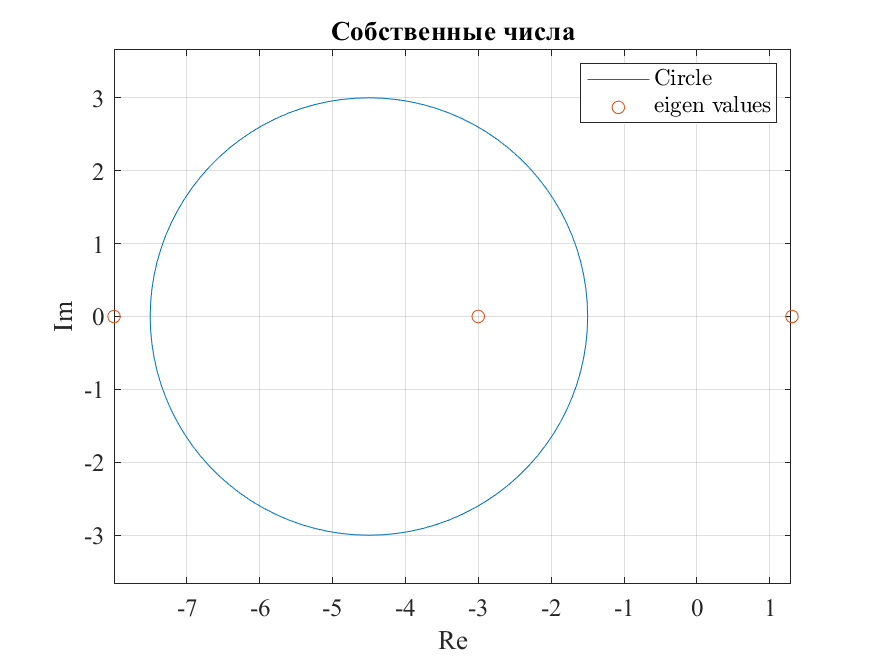
\includegraphics[width=0.8\textwidth]{plot_circle1.png}
  \caption{Проверка нахождения собственных чисел в пределах круга}
\end{figure}
\newpage
\begin{figure}[ht]
  \centering
  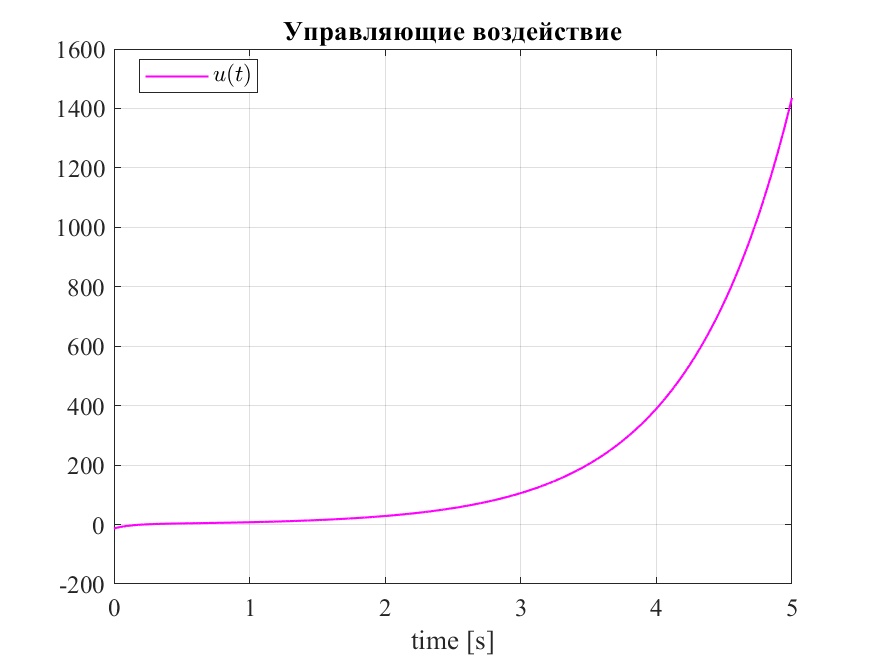
\includegraphics[width=0.8\textwidth]{ctrl_exp_u1.png}
  \caption{Моделирование - сигнал управления}
\end{figure}
\begin{figure}[ht]
  \centering
  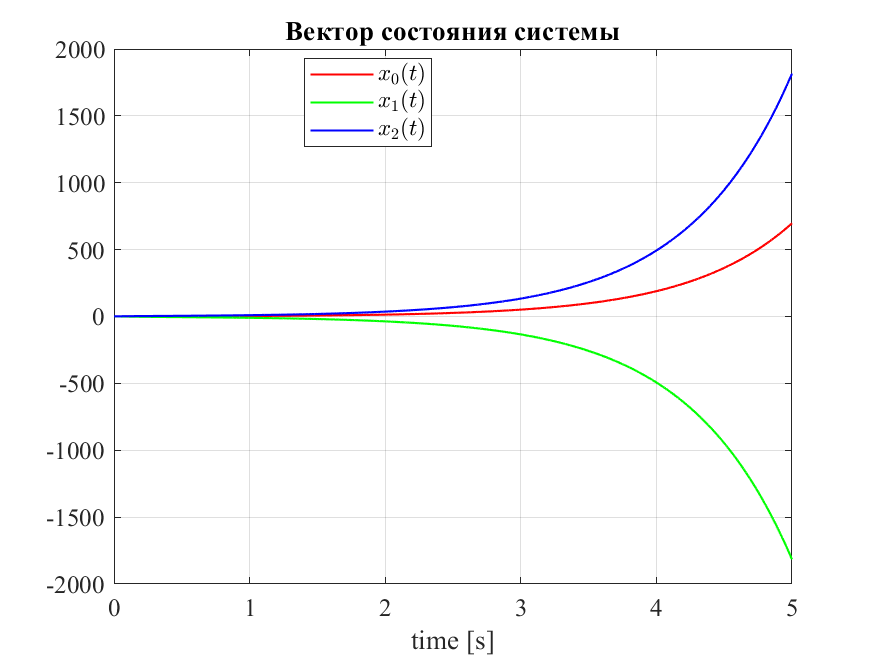
\includegraphics[width=0.8\textwidth]{ctrl_exp_x1.png}
  \caption{Моделирование - состояние системы}
\end{figure}
  

\newpage
\subsection{Второй набор Q и R}
$$Q=I, \tab R = 0$$

Решим  матричное уравнения типа Риккати:
$$
K_2 = \begin{bmatrix}
    1.38 & -2.31 & 1.38
\end{bmatrix}, \tab\rightarrow\tab \sigma(A+BK_2)=\{  -2.15 , -2.49,  -2 \}
$$

Можно заметить, что при таком наборе собственные числа находятся близко к $\lambda_3$.

\begin{figure}[ht]
  \centering
  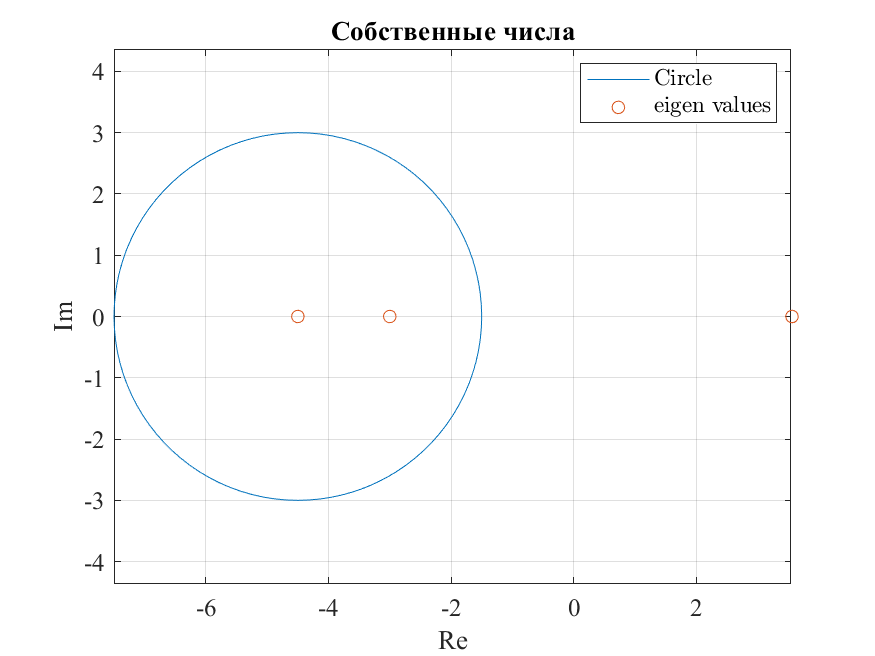
\includegraphics[width=0.8\textwidth]{plot_circle2.png}
  \caption{Проверка нахождения собственных чисел в пределах круга}
\end{figure}
\newpage
\begin{figure}[ht]
  \centering
  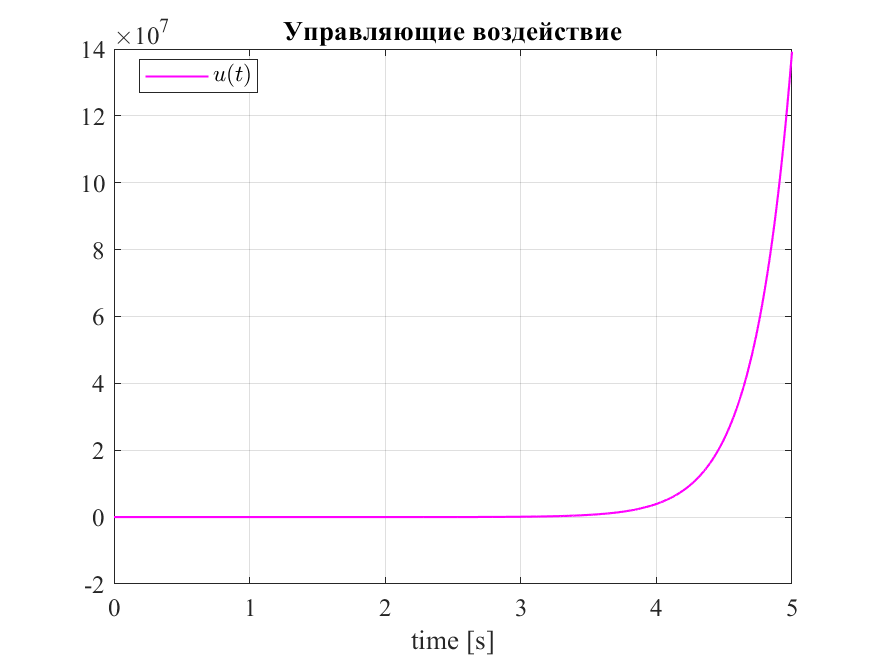
\includegraphics[width=0.8\textwidth]{ctrl_exp_u2.png}
  \caption{Моделирование - сигнал управления}
\end{figure}
\begin{figure}[ht]
  \centering
  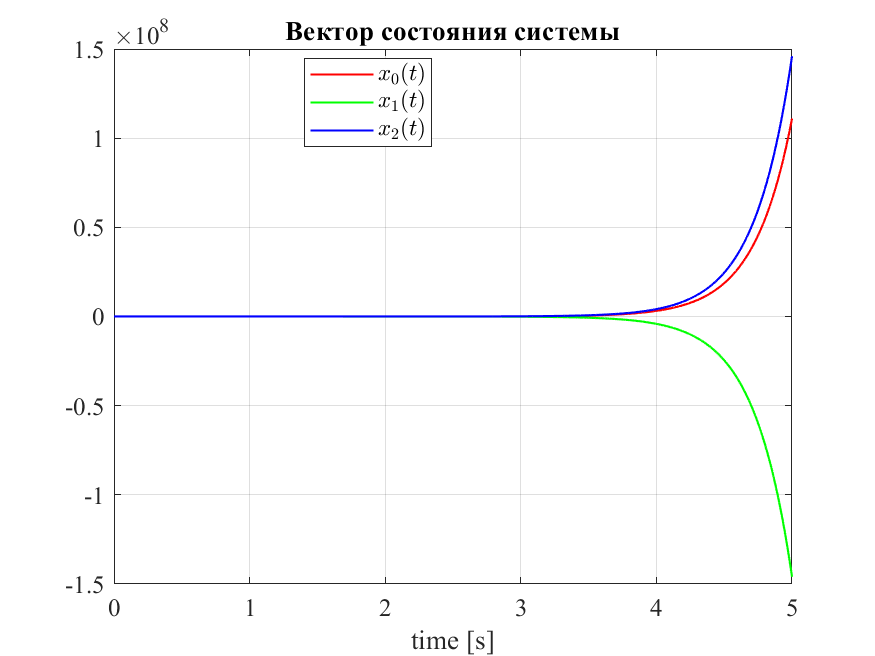
\includegraphics[width=0.8\textwidth]{ctrl_exp_x2.png}
  \caption{Моделирование - состояние системы}
\end{figure}

\newpage
\subsection{Третий набор Q и R}
$$Q=0, \tab R = 1$$

Решим  матричное уравнения типа Риккати:
$$
K_3 = \begin{bmatrix}
    1.39 & -3.75 & 1.39
\end{bmatrix}, \tab\rightarrow\tab \sigma(A+BK_3)=\{  -1.25 , -3.75,  -2 \}
$$

Можно заметить, мы получили вырожденный случай, два собственных числа лежат на окраине круга включительно:

\begin{figure}[ht]
  \centering
  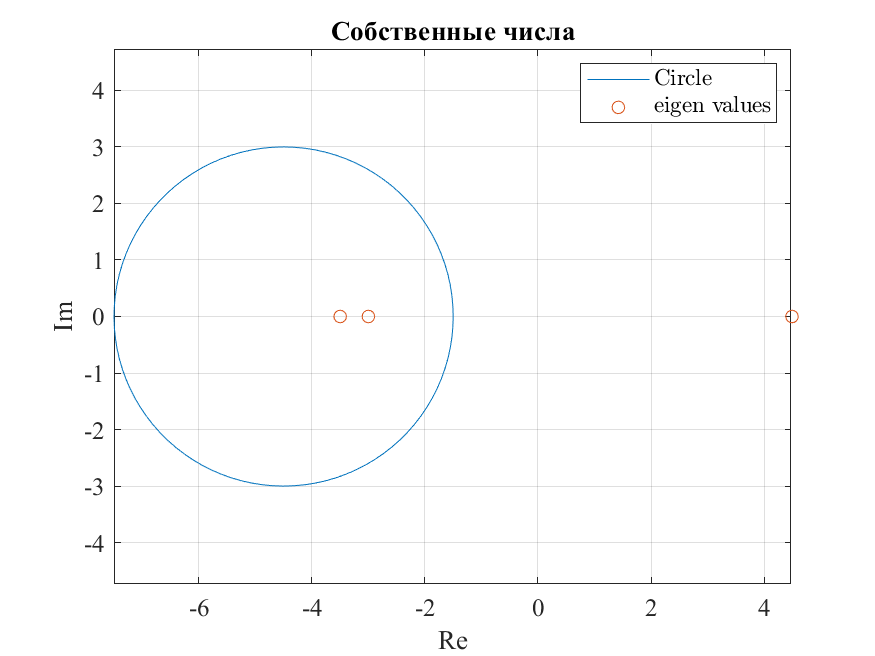
\includegraphics[width=0.8\textwidth]{plot_circle3.png}
  \caption{Проверка нахождения собственных чисел в пределах круга}
\end{figure}
\newpage
\begin{figure}[ht]
  \centering
  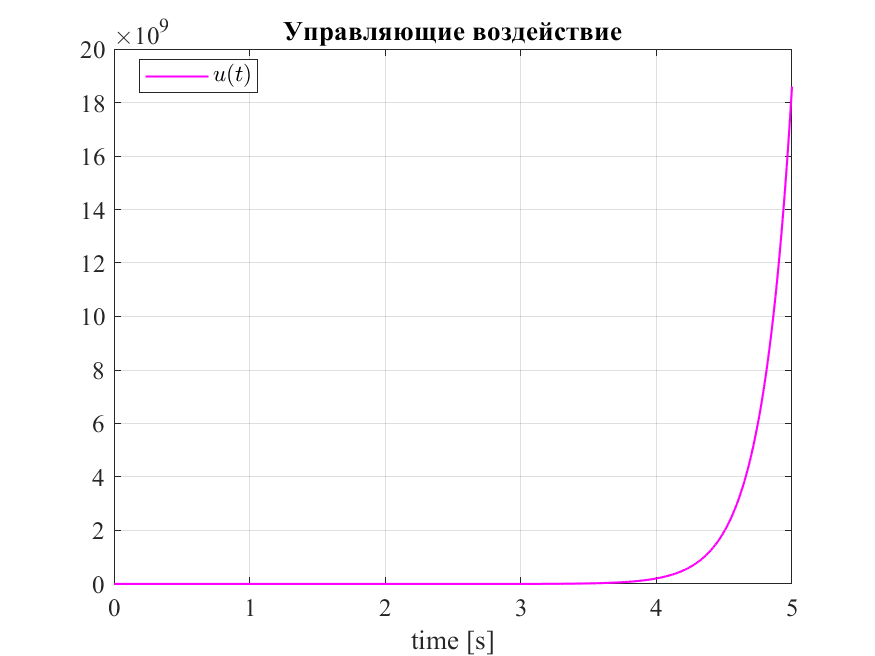
\includegraphics[width=0.8\textwidth]{ctrl_exp_u3.png}
  \caption{Моделирование - сигнал управления}
\end{figure}
\begin{figure}[ht]
  \centering
  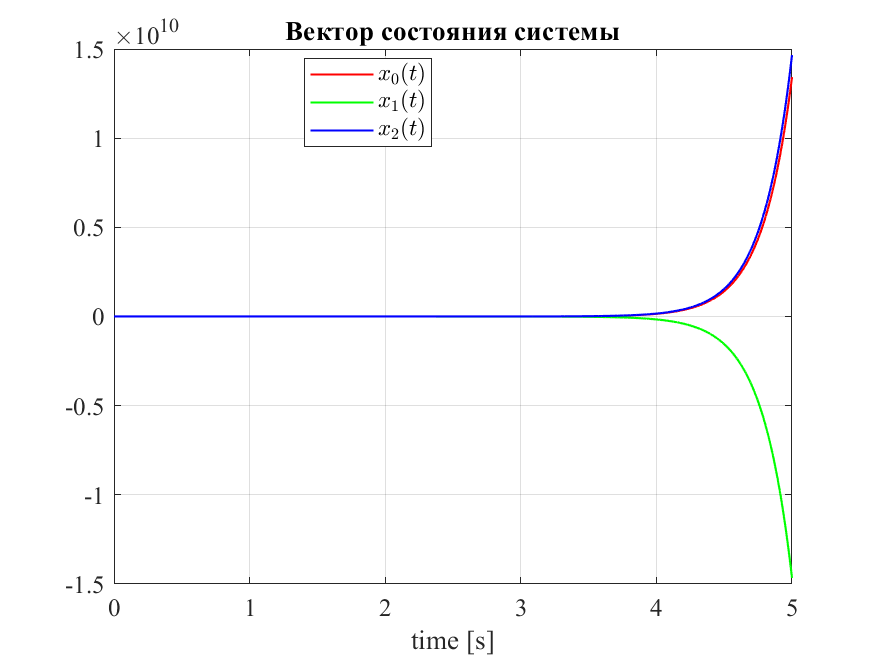
\includegraphics[width=0.8\textwidth]{ctrl_exp_x3.png}
  \caption{Моделирование - состояние системы}
\end{figure}

\newpage
\subsection{Четвертый набор Q и R}
$$Q=0, \tab R = 0$$

Решим  матричное уравнения типа Риккати:
$$
K_4 = \begin{bmatrix}
    1.1 & -2.07 & 1.1
\end{bmatrix}, \tab\rightarrow\tab \sigma(A+BK_4)=\{  -1.58 , -2.5,  -2 \}
$$


\begin{figure}[ht]
  \centering
  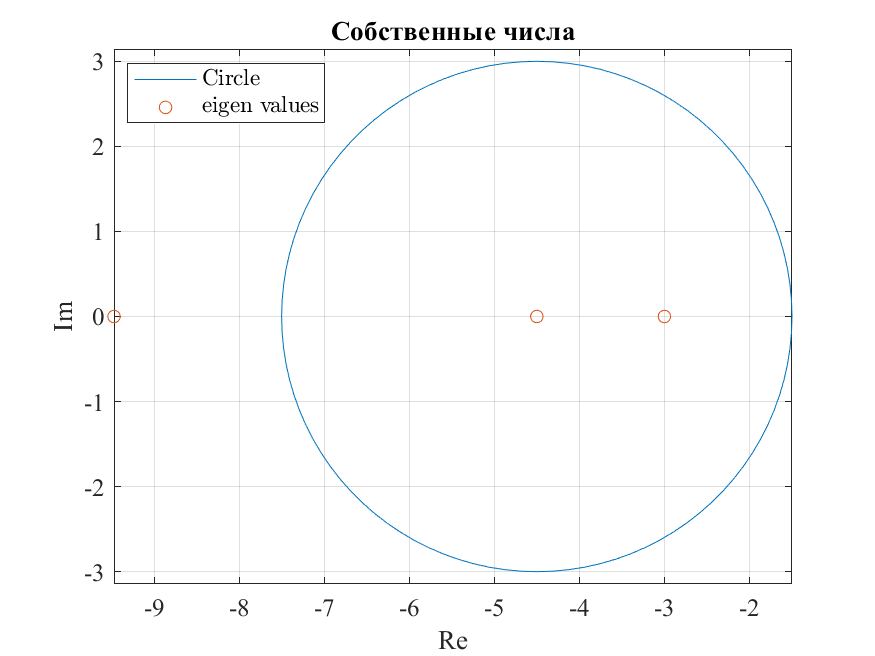
\includegraphics[width=0.8\textwidth]{plot_circle4.png}
  \caption{Проверка нахождения собственных чисел в пределах круга}
\end{figure}
\newpage
\begin{figure}[ht]
  \centering
  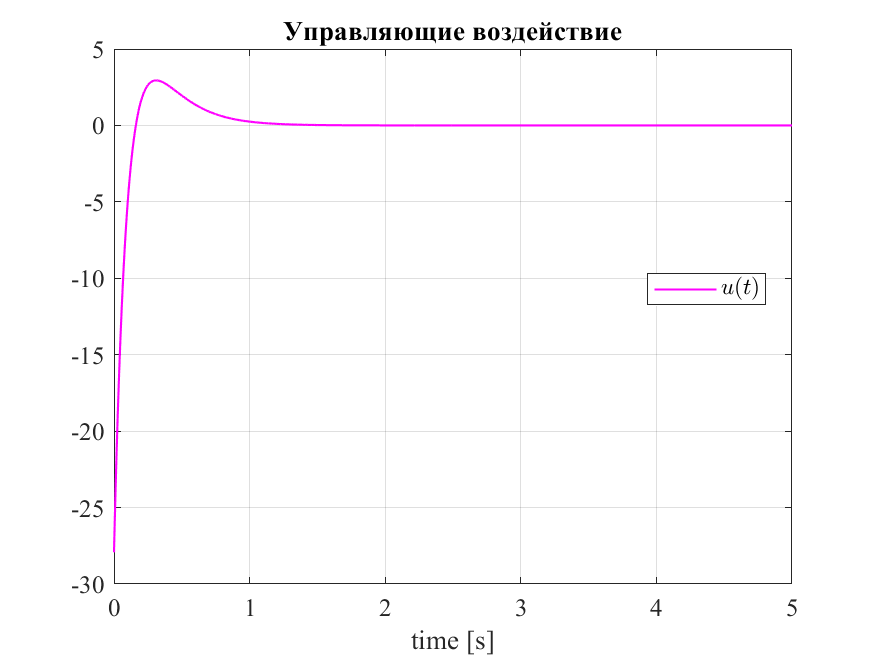
\includegraphics[width=0.8\textwidth]{ctrl_exp_u4.png}
  \caption{Моделирование - сигнал управления}
\end{figure}
\begin{figure}[ht]
  \centering
  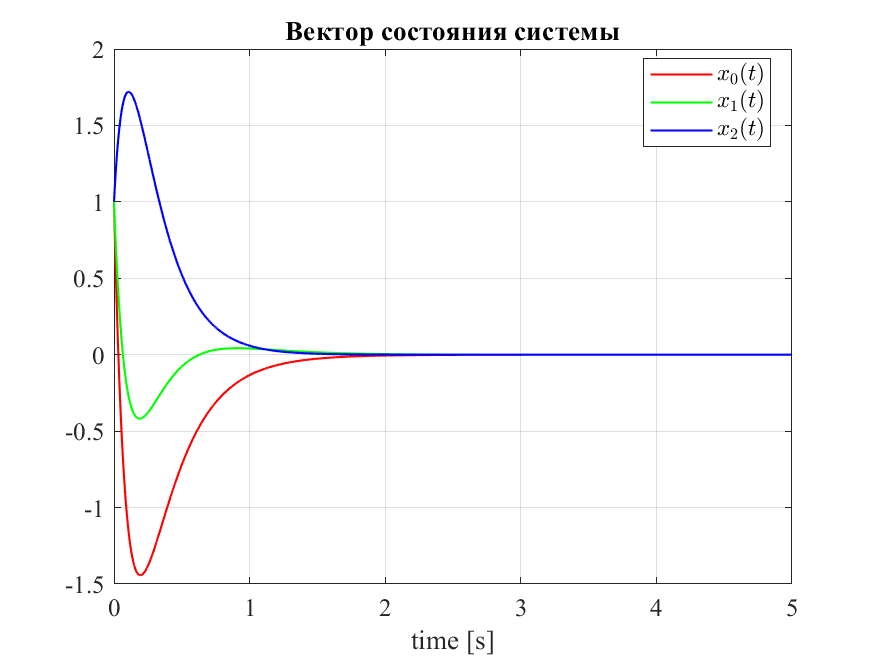
\includegraphics[width=0.8\textwidth]{ctrl_exp_x4.png}
  \caption{Моделирование - состояние системы}
\end{figure}

\newpage
Итоговые графики для сравнения:

\begin{figure}[ht]
  \centering
  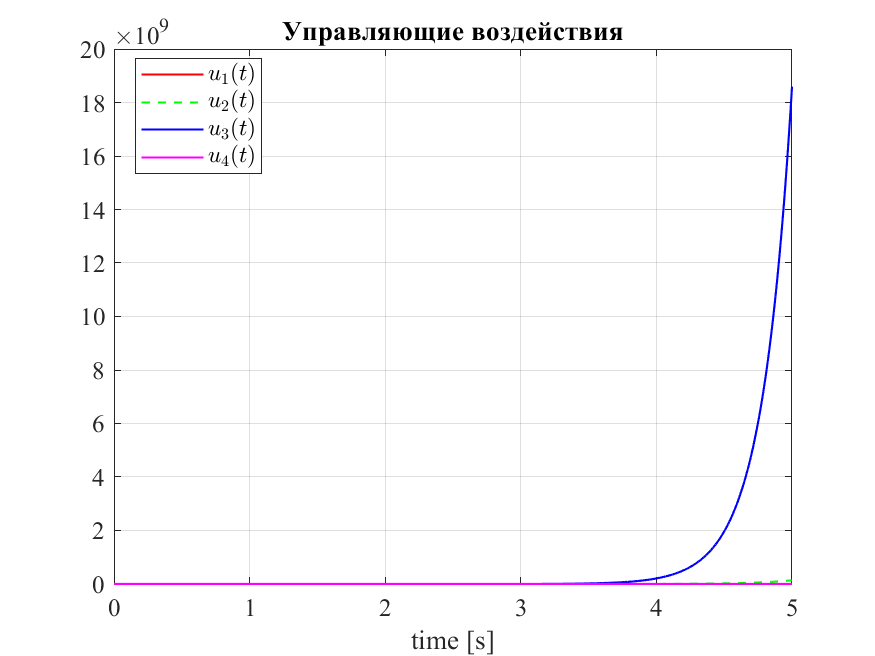
\includegraphics[width=0.8\textwidth]{ctrl_exp_u_all.png}
  \caption{Моделирование - сигналы управления}
\end{figure}
\begin{figure}[ht]
  \centering
  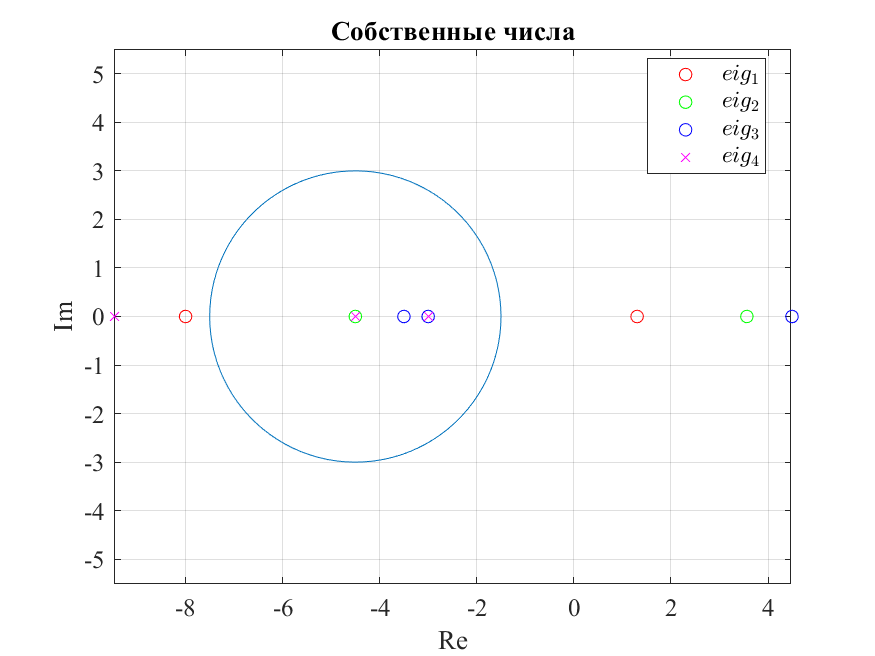
\includegraphics[width=0.8\textwidth]{plot_circle_all.png}
  \caption{Моделирование - все наборы собственных чисел}
\end{figure}
Получается, что настройка набором $Q, R$ давало довольно тонкие различия в управлении, поэтому в целом все четыре моделирования были почти идентичны.
\subsection{Вывод}
В этом задании мы синтезировали регулятор с качественной экспоненциальной устойчивостью для стабилизируемой системы.
При его настройки мы задавали средне желаемые значения устойчивости и возможные отклонения от неё, 
степень сходимости уже определял сам регулятор, с чем он успешно справился - при разных сочетаниях наборов $Q, R$ мы в среднем получили идентичный результат, регулятор отлично отработал.

\endinput